% This is samplepaper.tex, a sample chapter demonstrating the
% LLNCS macro package for Springer Computer Science proceedings;
% Version 2.21 of 2022/01/12
%
\documentclass[a4paper,UKenglish,hyperref,cleveref, autoref, thm-restate]{lipics-v2021}
%
\bibliographystyle{plainurl}% the mandatory bibstyle

\title{Robust Positivity Problems for low-order Linear Recurrence Sequences}
\titlerunning{Robust Positivity for low-order LRS}

\subtitle{The frontiers of decidability for explicitly given neighbourhoods}

\author{Mihir Vahanwala}{Max Planck Institute for Software Systems, Saarland Informatics Campus, Germany}{mvahanwa@mpi-sws.org}{https://orcid.org/0009-0008-5709-899X}{}

\authorrunning{M.\ Vahanwala} %TODO mandatory. First: Use abbreviated first/middle names. Second (only in severe cases): Use first author plus 'et al.'

\Copyright{M.\ Vahanwala} %TODO mandatory, please use full first names. LIPIcs license is "CC-BY";  http://creativecommons.org/licenses/by/3.0/

\ccsdesc[100]{Theory of computation; Logic and verification} %TODO mandatory: Please choose ACM 2012 classifications from https://dl.acm.org/ccs/ccs_flat.cfm 

\keywords{Dynamical Systems, Verification, Robustness, Linear Recurrence Sequences, Positivity, Ultimate Positivity}

%\nolinenumbers

\usepackage{amsfonts,stmaryrd,mathtools}
\usepackage{amsmath}
\usepackage{amssymb}
\usepackage{wrapfig}
% \usepackage{MnSymbol}
\usepackage[ruled,vlined,linesnumbered,titlenotnumbered,noend]{algorithm2e}
\usepackage{xcolor}
% \usepackage{paralist}
%% Some recommended packages.
\usepackage{booktabs}   %% For formal tables:
                        %% http://ctan.org/pkg/booktabs
\usepackage{subcaption} %% For complex figures with subfigures/subcaptions
                        %% http://ctan.org/pkg/subcaption
\captionsetup{compatibility=false}
\usepackage{pgf}
\usepackage{tikz}
\usepackage{listings}
% \usepackage[hmargin=1in]{geometry}
\usepackage[parfill]{parskip}
\usepackage[colorinlistoftodos,prependcaption,textsize=tiny]{todonotes}
\usepackage{float}
\usepackage{tcolorbox}
\usepackage{bbm}
% \usepackage{times}
\usepackage{hyperref}
\usepackage{cleveref}
\usepackage{lineno}


\newcommand{\rationals}{\mathbb{Q}}
\newcommand{\naturals}{\mathbb{N}}
\newcommand{\integers}{\mathbb{Z}}
\newcommand{\reals}{\mathbb{R}}
\newcommand{\complexes}{\mathbb{C}}
\newcommand{\algebraics}{\overline{\mathbb{Q}}}
\newcommand{\realalgebraics}{\mathbb{A}}
\newcommand{\field}{\mathbb{K}}
\newcommand{\ring}{\mathcal{O}}
\newcommand{\ideal}{\mathcal{I}}
\newcommand{\anideal}{\mathcal{J}}
\newcommand{\primeideal}{\mathfrak{p}}
\newcommand{\valuation}{v_\primeideal}
\newcommand{\pspace}{\mathsf{PSPACE}}
\newcommand{\conp}{\mathsf{coNP}}
\newcommand{\np}{\mathsf{NP}}
\newcommand{\pp}{\mathsf{PP}}

\newcommand{\seq}[1]{\langle#1\rangle}
\newcommand{\size}[1]{||#1||}

\newtheorem{problem}{Problem}
\usepackage{graphicx}

\begin{document}
\maketitle
\begin{abstract}
Linear Recurrence Sequences (LRS) are a fundamental mathematical primitive for a plethora of applications such as model checking, probabilistic systems, computational biology, and economics. Positivity (are all terms of the given LRS at least $0$?) and Ultimate Positivity (are all but finitely many terms of the given LRS at least $0$?) are important open number-theoretic decision problems. Recently, the robust versions of these problems, that ask whether the LRS is (Ultimately) Positive despite small perturbations to its initialisation, have gained attention as a means to model the imprecision that arises in practical settings. In this paper, we consider the neighbourhood as specified in the input of the robust decision problems. We contribute by proving sharp decidability results: in each case, decidability at orders our techniques can't handle would entail significant number-theoretic breakthroughs.
\end{abstract}
\section{Introduction}
\label{section:intro}
A real Linear Recurrence Sequence (LRS) of order $\kappa$ is an infinite sequence of real numbers $\seq{u_0, u_1, u_2, \dots}$ having the following property: there exist $\kappa$ real constants $a_{0}, \dots, a_{\kappa-1}$, with $a_0 \ne 0$ such that for all $n \ge 0$:
\begin{equation}
u_{n+\kappa} = a_{\kappa-1}u_{n+\kappa-1} + \dots a_0 u_n
\end{equation}
An LRS is uniquely specified given the constants $a_0, \dots, a_{\kappa-1}$, and the initial terms $u_0, \dots, u_{\kappa-1}$. The best-known example is the Fibonacci sequence $\seq{0, 1, 1, 2, 3, 5, 8, \dots}$, satisfying the recurrence relation $u_{n+2} = u_{n+1} + u_n$: it is named after Leonardo of Pisa, who used it to model the population growth of rabbits. LRS have been extensively studied, and found several mathematical and scientific applications since. The monograph of Everest \textit{et al.} \cite{Everest2003RecurrenceS} is a comprehensive treatise on the mathematical aspects of Recurrence Sequences.

Important number-theoretic decision problems for Linear Recurrence Sequences include Positivity (is $u_n \ge 0$ for all $n$?), Ultimate Positivity (is $u_n \ge 0$ for all but finitely many $n$?) and the Skolem Problem (is $u_n = 0$ for some $n$?). These problems have applications in software verification, probabilistic model checking, discrete dynamic systems, theoretical biology, and economics. Decidability has been open for decades: Ouaknine and Worrell \cite{joeljames3} showed Positivity and Ultimate Positivity are decidable up to order $5$ but number-theoretically hard at order $6$, whereas Mignotte \textit{et al.} \cite{mignotte} and Vereshchagin \cite{vereshchagin} independently proved the Skolem Problem to be decidable up to order $4$. These results were proven given the \textit{rational} $a_0, \dots, a_{\kappa-1}, u_0, \dots u_{\kappa-1}$ as input, but can be generalised to real algebraic input as well. In this paper, we focus on Positivity and Ultimate Positivity for real algebraic sequences.

In contrast, the \textit{uninitialised} variants of these problems are far more tractable. \cite{Braverman06,Tiwari04} consider whether \textit{every} possible initialisation keeps the sequence Positive, and decide so in $\mathsf{PTIME}$. More recently, this result has been extended to processes with choices \cite{AGV18}. We argue that practical applications need a middle ground: recurrence relations that arise in practice need to be contextualised by actual instances of sequences; however, considering \textit{precise} initialisations does not account for inherently imprecise real world measurements, and the requirement of safety margins. We thus study robust variants: given a recurrence and an initialisation, do all initialisations in a neighbourhood satisfy (Ultimate) Positivity?

\subsubsection*{Related Work} 
In this paper, we focus on the neighbourhood-of-initialisation notion of robustness, which was first introduced in \cite{originalstacs}, and more comprehensively treated in \cite{originalarxiv}. There are, however, different approaches to tackle imprecision: \cite{N21} considers a model of computation that can take arbitrary real numbers as input. Works with a more control-theoretic flavour include \cite{rounding20}, which allows for rounding at every step before applying the recurrence; in the same vein, \cite{pseudo21} allows for $\varepsilon$-disturbances at every step. Our notion of robustness has been considered in \cite{originalstacs,originalarxiv,pseudo21}, however, these works primarily concern themselves with simply deciding whether there \textit{exists} a neighbourhood around the given point that satisfies Positivity. Although they do identify that robust problems are hard when the neighbourhood is given as input, in the absence of decidability results, their hardness results are not sharp.

\subsubsection*{Our contribution}
We address the gap in the robustness state-of-the-art by exploring the frontiers of decidability when the neighbourhood is given as input. In \S\ref{section:solspace} we define the robustness problems we consider: we use the Mahalanobis distance to specify neighbourhoods. Our parameter is the positive definite matrix $\mathbf{S}$, and the neighbourhood of $\mathbf{c}$ it specifies is the set of all points $\mathbf{c'} \in \reals^{\kappa}$ such that $\sqrt{(\mathbf{c'} - \mathbf{c})^T\mathbf{S}(\mathbf{c'} - \mathbf{c})} \le 1$. In the statistical context, $\mathbf{S}$ is the inverse of a covariance matrix; and thus, our formulation is a rather natural way of capturing noise and measurement errors in the input. Our \textbf{novelty}, to the best of our knowledge, lies in identifying a general and practical way of explicitly specifying neighbourhoods, and establishing the \textbf{first decidability results} in such a setting, albeit at low orders. We prove these results in \S\ref{section:decidability} and \S\ref{section:decidability2}. In \S\ref{section:hardness}, we show how the number-theoretic hardness we formalise in \S\ref{section:diophantine} rears its head at immediately higher orders. Our contributions are summarised in the table below.
\begin{table}[H]
\begin{tabular}{|l|c|r|}
  \hline
   \textbf{Robust Problem}& \textbf{Decidability }& {\bf Hardness} \\
  \hline
  $\mathbf{S}$-Robust Positivity & Up to order 4 & Diophantine hard at order 5\\
  $\mathbf{S}$-Robust Uniform Ultimate Positivity & Up to order 4 & Lagrange hard at order 5 \\
  $\mathbf{S}$-Robust Non-uniform Ultimate Positivity & Up to order 5 & (\cite{originalarxiv,joeljames3}) Lagrange hard at order 6 
  \\
  \hline
\end{tabular}

\caption{Problems are as formally defined in \S\ref{section:solspace}. The distinction between uniform and non-uniform refers to whether the threshold index for certifying Ultimate Positivity must be common for the entire neighbourhood. Hardness results are in the sense of Definition \ref{def:hardness}.}% 
  \label{tab:results}
\end{table}

\subsubsection*{Notation and Prerequisites}
For the purposes of discussing robustness, we shall use $\ball$ to denote the unit ball in $\reals^\kappa$, centred at the origin. Similarly, we use $\ball_{\mathbf{S}}$ to denote the set of $\mathbf{d}$ such that $\mathbf{d}^T\mathbf{Sd} \le 1$. For real column vectors $\mathbf{x}, \mathbf{y}$, we use $\seq{\mathbf{x}, \mathbf{y}}$ to denote the inner product $\mathbf{x}^T\mathbf{y} = \mathbf{y}^T\mathbf{x}$. $||\mathbf{x}||$ denotes the standard L2 norm $\sqrt{\seq{\mathbf{x}, \mathbf{x}}}$

Throughout this paper,  $\naturals$, $\integers$, $\rationals$, $\reals$, and $\complexes$ respectively denote the natural numbers, integers, rationals, reals, and complex numbers. $\alpha \in \complexes$ is said to be algebraic if it is a root of a polynomial with integer coefficients. Algebraic numbers form an algebraically closed field, denoted by $\algebraics$. We denote the field of real algebraic numbers by $\realalgebraics$.

In this paper, we assume our input consists of real algebraic numbers. Appendix \ref{appendix:prelims} contains a brief initiation to this number field. The key takeaways are that the usual arithmetic can be carried out with perfect precision, and that the First Order Theory of the Reals $\seq{\reals; +, \cdot, \ge, 0, 1}$ is a decidable logical system powerful enough to fit our purposes.

\begin{theorem}[Renegar \cite{renegar}]
\label{thm:renegar}
Let $M \in \naturals$ be fixed. Let $\chi(\mathbf{x})$ be a First Order Logic formula interpreted over the reals with fewer than $M$ variables in total. There exists a procedure that returns an equivalent quantifier-free formula $\psi(\mathbf{x})$ in disjunctive normal form. This procedure runs in time polynomial in the size of the representation of $\chi$.
\end{theorem} 




\section{Linear Recurrences and Robustness}
\label{section:solspace}

We start approaching robustness by formally decoupling the elements of an LRS: namely, the recurrence relation, and the initialisation.

\begin{definition}[Linear Recurrence Relation (LRR)]
\label{def:LRR}
A real algebraic LRR $\mathbf{a}$ of order $\kappa$:
\begin{itemize}
\item is a $\kappa+1$-ary relation, specified by $\kappa$ numbers, $a_0, \dots, a_{\kappa-1} \in \realalgebraics$, with $a_0 \ne 0$. $\mathbf{a}(Y_0, Y_1, \dots, Y_\kappa)$ is interpreted as 
$
Y_\kappa = \sum_{j=0}^{\kappa-1} a_j Y_j
$.
\item has a characteristic polynomial is
$
X^{\kappa} - \sum_{j=0}^{\kappa-1}a_j X^j
$.
\end{itemize}
\end{definition}

\begin{definition}[Linear Recurrence Sequence (LRS)]
\label{def:LRS}
A real algebraic LRS $\mathbf{u}$ of order $\kappa$ is an infinite sequence $\seq{u_n}_{n=0}^\infty$, given by a real algebraic order $\kappa$ LRR $\mathbf{a}$ and the initialisation $\mathbf{c} = (u_0, u_1, \dots, u_{\kappa-1}) \in \realalgebraics^\kappa$. For all $n \in \naturals$, $\mathbf{a}(u_n, u_{n+1}, \dots, u_{n+\kappa})$ holds.
\end{definition}

One can also encode the recurrence $\mathbf{a}$ as a $\kappa \times \kappa$ companion matrix $\mathbf{A}$, and interpret the initialisation $\mathbf{c}$ as a vector. Then, $u_n$ is given by the first coordinate of $\mathbf{A}^n\mathbf{c}$, i.e.
\begin{equation}
\label{eq:companion}
\begin{bmatrix}
u_n \\
u_{n+1} \\
\vdots \\
u_{n+\kappa-1}
\end{bmatrix} 
= 
\begin{bmatrix}
0 & 1 & 0 & \dots & 0 \\
0 & 0 & 1 & \dots & 0 \\
\vdots & \vdots & \vdots & \dots & \vdots \\
a_0 & a_1 & a_2 & \dots & a_{\kappa-1}
\end{bmatrix}^n
\begin{bmatrix}
u_0 \\
u_{1} \\
\vdots \\
u_{\kappa-1}
\end{bmatrix}.
\end{equation}
Let $\mathbf{e_1}^T$ denote the row vector $\begin{bmatrix}1 & 0 & \dots & 0\end{bmatrix}$. We can thus write $u_n = \mathbf{e_1}^T\mathbf{A}^n\mathbf{c}$. It is now a standard fact that LRS have the following \textbf{real exponential polynomial} closed form
\begin{equation}
\label{eq:realexppoly}
u_n = \left(\sum_{j=1}^{k_1}\sum_{\ell = 0}^{m_j-1} z_{j\ell}\rho_j^n n^\ell\right) + \left(\sum_{j=k_1 + 1}^{k_2} \sum_{\ell = 0}^{m_j-1} (x_{j\ell} \cos n\theta_j + y_{j\ell}\sin n\theta_j)\rho_j^n n^\ell\right)
\end{equation}
where $\rho_j$ (alternately, $\rho_j e^{i\theta_j}$) are roots of the characteristic polynomial defined by $\mathbf{a}$, each with multiplicity $m_j$. The coefficients $z_{j\ell}, x_{j\ell}, y_{j\ell}$ each depend linearly on $\mathbf{c}$. Roots such that $|\rho_j|$ is the largest are called \textbf{dominant}. The growth rate of a term in the above expression is governed by $\rho_j^n n^\ell$. Terms with the fastest growth are called \textbf{dominant terms}, and they drive the asymptotic behaviour of the LRS.

Throughout this paper, we consider that our input consists of real algebraic numbers.
An LRS $\seq{u_n}_{n=0}^\infty$ is given as $(\mathbf{a}, \mathbf{c})$, i.e. the real algebraic recurrence and the initialisation. The Positivity problem is to decide whether for all $n \in \naturals$, $u_n \ge 0$.
The Ultimate Positivity problem is to decide whether there exists an $N$ such that for all $n \ge N$, $u_n \ge 0$.


A Positive LRS is necessarily Ultimately Positive. As alluded to in the Introduction, \cite{joeljames3} shows both Positivity and Ultimate Positivity to be decidable up to order 5, while demonstrating number-theoretic hardness at order 6 in the precise sense of Definition \ref{def:hardness}. On restricting our attention to \textit{simple} LRS (the characteristic polynomial has no repeated root), Positivity is decidable up to order 9 \cite{ouaknine2014positivity}, while Ultimate Positivity is decidable at all orders \cite{ouaknine2014ultimate}. In this paper, we shall focus on defining and tackling robust versions of these problems.

In all the problems we consider, our input consists of a linear recurrence relation $\mathbf{a}$, an initialisation $\mathbf{c}$, and a positive definite matrix $\mathbf{S}$ that is used to define a neighbourhood around $\mathbf{c}$. All input is made up of real algebraic entries.

\begin{problem}[$\mathbf{S}$-Robust Positivity]
\label{prob:rrobpos}
Decide whether for all $\mathbf{c'}$ such that $(\mathbf{c'} - \mathbf{c})^T\mathbf{S}(\mathbf{c'} - \mathbf{c}) \le 1$, the LRS $(\mathbf{a}, \mathbf{c'})$ is positive.
\end{problem}

\begin{problem}[$\mathbf{S}$-Robust Uniform Ultimate Positivity]
\label{prob:rrobuniultpos}
Decide whether there exists an $N$ such that for all $\mathbf{c'}$ with $(\mathbf{c'} - \mathbf{c})^T\mathbf{S}(\mathbf{c'} - \mathbf{c}) \le 1$, the LRS $(\mathbf{a}, \mathbf{c'})$ is positive from the $N^{th}$ term onwards.
\end{problem}

We can switch the order in which $N$ and $\mathbf{c'}$ are quantified, and query a weaker notion of Robust Ultimate Positivity:
\begin{problem}[$\mathbf{S}$-Robust Non-uniform Ultimate Positivity]
\label{prob:rrobnonuniultpos}
Decide whether for all $\mathbf{c'}$ with $(\mathbf{c'} - \mathbf{c})^T\mathbf{S}(\mathbf{c'} - \mathbf{c}) \le 1$ , there exists an $N$ such that the LRS $(\mathbf{a}, \mathbf{c'})$ is positive from the $N^{th}$ term onwards.
\end{problem}

The attentive reader might have already noticed that we depart from convention and specify neighbourhoods as \textit{closed} balls. Although \cite{originalarxiv} does not solve the problems we consider in this paper, it makes crucial observations about the geometry: for Problems \ref{prob:rrobpos} and \ref{prob:rrobuniultpos}, there is no difference between open and closed balls. On the other hand, Problem \ref{prob:rrobnonuniultpos} becomes considerably easier with open balls, and its decidability assuming open balls is tackled in \cite{originalarxiv} itself. 

In general, an arbitrary point $\mathbf{c'}$ is expressed as $\mathbf{c} + \mathbf{d}$, where $\mathbf{d} \in \mathcal{P}$, a full-dimensional neighbourhood symmetric about the origin. Observe equation \ref{eq:companion}. The $n^{th}$ term of the LRS is non-negative throughout the neighbourhood if and only if for all $d \in \mathcal{P}$
\begin{equation}
\mathbf{e_1}^T \mathbf{A}^n (\mathbf{c + d}) \ge 0.
\end{equation}
We can use the symmetry of $\mathcal{P}$ about the origin to rewrite the above as
\begin{equation}
\label{eq:illustrate}
\mathbf{e_1}^T \mathbf{A}^n \mathbf{c}\ge \max_{\mathbf{d} \in \mathcal{P}} \mathbf{e_1}^T\mathbf{A}^n\mathbf{d} \ge 0.
\end{equation}
\textbf{The overview of our approach to Problems \ref{prob:rrobpos} and \ref{prob:rrobuniultpos} is as follows.}
\begin{enumerate}
\item Constructively decide whether there exists an $N_1$ such that $\mathbf{e_1}^T \mathbf{A}^n \mathbf{c} \ge 0$ for all $n > N_1$. Given the LRS $(\mathbf{a}, \mathbf{c})$ as input, this is precisely the core capability of decision procedures for Positivity problems for LRS up to order 5, presented in \cite{joeljames3}.
\item Use linear-algebraic arguments to define LRS $(v_n)_{n=0}^\infty$, such that $v_n \ge 0$ if and only if $|\mathbf{e_1}^T \mathbf{A}^n \mathbf{c}|\ge \max_{\mathbf{d} \in \mathcal{P}} \mathbf{e_1}^T\mathbf{A}^n\mathbf{d}$.
\item Constructively decide whether there exists $N_2$ such that $v_n \ge 0$ for all $n > N_2$. Positivity throughout the neighbourhood is thus guaranteed beyond step $N = \max(N_1, N_2)$.
\item Explicitly check inequality \ref{eq:illustrate} for $n \le N$.
\end{enumerate}

Step 2 and the executability of Step 3 in low dimensions form the crux of our novelty. As a simple illustration, assume that the neighbourhood is defined by a polytope rather than a positive definite matrix. This situation arises, for instance, when the metric is based on the $\ell^1$- or $\ell^\infty$-norm, as opposed to the $\ell^2$-norm.  In this simple example, $\mathcal{P}$ is a polytope, hence $\mathbf{e_1}^T\mathbf{A}^n\mathbf{d}$ is maximised at one of the finitely many corners $\{\mathbf{d_1}, \dots, \mathbf{d_k}\}$. Thus, steps 2 and 3 amount to using \cite{joeljames3} again to check the (Ultimate) Positivity of each of the low-order LRS $(\mathbf{a}, \mathbf{c+d_i})$.

We now discuss how we perform Step 2 when $\mathcal{P} = \mathcal{B}_\mathbf{S}$, a neighbourhood of vectors $\mathbf{d}$ such that $\mathbf{d}^T\mathbf{S}\mathbf{d} \le 1$. The defining parameter $\mathbf{S}$ is a real algebraic positive definite matrix. We note that since $\mathbf{S}$ is positive definite, it can be factored as $\mathbf{G}^T\mathbf{G}$, where $\mathbf{G}$ is a real algebraic invertible matrix. We denote $\mathbf{Gd} = \mathbf{f}$. We argue that $\mathbf{G}^{-1}$ bijectively maps the Euclidean unit ball $\mathcal{B}$ to $\mathcal{B}_\mathbf{S}$. The bijection is clear from the invertibility of the matrix. Suppose $\mathbf{d} = \mathbf{G}^{-1}\mathbf{f}$, where $\mathbf{f} \in \mathcal{B}$, i.e. $\mathbf{f}^T\mathbf{f} \le 1$. Then $\mathbf{d}^T\mathbf{Sd} = \mathbf{d}^T\mathbf{G}^T\mathbf{Gd} = \mathbf{f}^T\mathbf{f} \le 1.$
Therefore,
\begin{equation}
\max_{\mathbf{d} \in \mathcal{B}_\mathbf{S}} \mathbf{e_1}^T\mathbf{A}^n\mathbf{d} = \max_{\mathbf{f} \in \mathcal{B}} \mathbf{e_1}^T\mathbf{A}^n\mathbf{G}^{-1}\mathbf{f}.
\end{equation}
$\mathcal{B}$ is a convex set; thus a linear function will necessarily be maximised at its boundary, i.e. when $||\mathbf{f}|| = 1$. The linear function $\mathbf{h}^T\mathbf{f}$ is maximised over the unit Euclidean ball when $\mathbf{f}$ is aligned along $\mathbf{h}$; the maximum value is $||\mathbf{h}||$. Thus
\begin{equation}
\max_{\mathbf{d} \in \mathcal{B}_\mathbf{S}} \mathbf{e_1}^T\mathbf{A}^n\mathbf{d} = \left|\left|\left( \mathbf{e_1}^T\mathbf{A}^n\mathbf{G}^{-1} \right)^T\right|\right|.
\end{equation}

In order to express a necessary and sufficient condition for $|\mathbf{e_1}^T \mathbf{A}^n \mathbf{c}|\ge \max_{\mathbf{d} \in \mathcal{P}} \mathbf{e_1}^T\mathbf{A}^n\mathbf{d}$ to hold in terms of the positivity of an LRS at step $n$, we simply square both sides of the inequality, and transfer all terms to the left: 
\begin{equation}
(\mathbf{e_1}^T \mathbf{A}^n \mathbf{c})^2 - (\mathbf{e_1}^T \mathbf{A}^n \mathbf{g_1})^2 - \dots - (\mathbf{e_1}^T \mathbf{A}^n \mathbf{g_\kappa})^2 \ge 0.
\end{equation}
Crucially, $\mathbf{g_1}, \dots, \mathbf{g_\kappa}$ are the linearly independent columns of the invertible $\mathbf{G}^{-1}$. In \S\ref{section:decidability}, we give the technical details of how Step 3 of the above plan can be implemented, thus proving our first main decidability result.

\begin{theorem}[First Main Decidability Result]
\label{thm:decide}
Problems \ref{prob:rrobpos} and \ref{prob:rrobuniultpos} are decidable up to order 4.
\end{theorem}

\textbf{Our strategy for Problem \ref{prob:rrobnonuniultpos} is as follows.}
\begin{enumerate}
\item Consider the invertible matrix $\mathbf{V}^{-1}$ that maps initialisations to the coefficients in the real exponential polynomial closed form \ref{eq:realexppoly}.
\item Define $\mu(\mathbf{c})$ to be the (normalised) greatest lower bound for the contribution from the dominant terms corresponding to $\mathbf{c}$.
\item Use the First Order Theory of the Reals to check that $\mu(\mathbf{c'}) \ge 0$ for all $\mathbf{c'}$ in the given neighbourhood, and detect the critical boundary cases when $\mu(\mathbf{c'}) = 0$.
\item Exploit the low dimensionality to handle the critical boundary cases when $\mu(\mathbf{c'}) = 0$.
\end{enumerate}

We adopt this strategy and prove our second decidability result in \S\ref{section:decidability2}.
\begin{theorem}[Second Decidability Result]
\label{thm:decide2}
Problem \ref{prob:rrobnonuniultpos} is decidable up to order 4.
\end{theorem}






\section{Diophantine Approximation}
\label{section:diophantine}

Diophantine Approximation is a vast and active number-theoretic field of research concerned, among other things, with the approximation of reals by rational numbers. In this section, we follow Lagarias and Shallit’s terminology \cite{dio-constants} and briefly introduce classes of constants whose computation is an open problem. In what follows, $[x]$ denotes the shortest distance from $x$ to an integer; while $[x]_b$ denotes the shortest distance from $x$ to an integer multiple of $b$. $[x]_b = b[x/b]$

\begin{definition}[Diophantine Approximation Type]
\label{def:L}
The homogenous Diophantine approximation type $L(t)$ is defined to be $\inf_{n \in \naturals \backslash{0}} n[nt]$. The inhomogeneous Diophantine approximation type $L(t, s)$ is defined to be $\inf_{n \in \naturals \backslash{0}} n[nt - s]$, $s \notin \integers + t\integers$. 
\end{definition} 

\begin{definition}[Lagrange constant]
\label{def:Linfty}
The homogenous Lagrange constant $L_\infty(t)$ is defined to be $\liminf_{n \in \naturals} n[nt]$. The inhomogeneous Lagrange constant $L_\infty(t, s)$ is defined to be\\ $\liminf_{n \in \naturals} n[nt - s]$, $s \notin \integers + t\integers$.
\end{definition} 

It is known (Dirichlet, Minkowski \cite{minkowski}) that these constants lie between $0$ and $1$. As an immediate corollary, one observes that
\begin{equation}
\label{eq:quadraticdecay}
\exists c.~\forall t, s.~ \exists^\infty n. ~ 1 - \cos(nt - s) \le \frac{1}{2}\left[nt - s \right]_{2\pi}^2 \le \frac{c}{n^2}
\end{equation}

We record a useful number-theoretic fact: its proof relies on the Ostrowski numeration system \cite{bourla2016ostrowski,berthe2022dynamics}, and is deferred to Appendix \ref{appendix:ostrowski}.
\begin{lemma}
\label{lemma:existsreal}
For every irrational number $x$, strictly decreasing real positive function $\psi$, and interval $\mathcal{I} = [a, b] \subset [0, 1], ~ a \ne b$, there exists $y \in \mathcal{I}$ such that $[nx - y] < \psi(n)$ for infinitely many odd, and infinitely many even $n$.
\end{lemma}

Following \cite{joeljames3}, we note that the Diophantine approximation type and Lagrange constant of most transcendental numbers are unknown, and define
\begin{equation}
\mathcal A=\{p+q i \in \mathbb{C} \mid p,q \in \mathbb{A}, p^2+q^2=1, \forall n.~(p + qi)^n \ne 1\}
\end{equation}
i.e., the set of points on the unit circle of $\mathbb{C}$ with rational real and imaginary parts, excluding $1,-1, i$ and $-i$. The set $\mathcal A$ consists of algebraic numbers, none of which are roots of unity. In particular, writing $p+q i= e^{i 2 \pi \theta}$, we have that $\theta \notin \mathbb{Q}$. We denote:
\begin{equation}
\label{eq:keyset}
\mathcal{T} = \left\{ \theta \in (- 1/2, 1/2] \mid e^{2 \pi i \theta} \in \mathcal{A}\right\}
\end{equation}
The set $\mathcal{T}$ is dense in $(- \frac 1 2, \frac 1 2]$. In general, we don't have a method to compute $L(\theta)$ or $L_\infty(\theta)$ for $\theta \in \mathcal{T}$, or approximate them with arbitrary precision.

\begin{definition}[Number-theoretic hardness]
\label{def:hardness}
Let $\mathcal{T}$ be as above. A decision problem is said to be $\mathcal{T}$-Diophantine hard (resp.\ $\mathcal{T}$-Lagrange hard), if its decidability entails that given any $t \in \mathcal{T}$ and $\varepsilon > 0$, one can compute $\ell$ such that $|\ell - L(t)| < \varepsilon$ (resp.\  $|\ell - L_\infty(t)| < \varepsilon$).
\end{definition}

\begin{theorem}[Main Hardness Result]
\label{thm:hardness}
Problem \ref{prob:rrobpos} (resp.\ Problem \ref{prob:rrobuniultpos}) is $\mathcal{T}$-Diophantine hard (resp.\ $\mathcal{T}$-Lagrange hard) at order 5. 
\end{theorem}

\cite{originalarxiv} notes that in view of the Lagrange hardness (Definition \ref{def:hardness}) of Ultimate Positivity at order 6 \cite{joeljames3}, Problem \ref{prob:rrobnonuniultpos} is also Lagrange hard at order 6: one can simply construct a neighbourhood that lies entirely in the region $\mu > 0$ (i.e. neighbourhoods for which Ultimate Positivity can be \textit{certified}), except for a hard instance of Ultimate Positivity on its surface. In this way, Ultimate Positivity is guaranteed for all but the single critical point on the boundary.

\begin{theorem}
\label{thm:hardness2}
Problem \ref{prob:rrobnonuniultpos} is $\mathcal{T}$-Lagrange hard at order 6. 
\end{theorem}






\section{Uniform Robustness: Decidability at order four}
\label{section:decidability}

%\begin{theorem}[Masser \cite{Masser}]
  \label{thm:abelian}
 % Let $e^{i \theta_1},...,e^{i \theta_k}$ be complex algebraic numbers of unit modulus. Consider the free abelian group $L$ defined by $L = \{(\lambda_1, \ldots ,\lambda_k) \in \mathbb{Z}^k: 
 % e^{i (\lambda_1 \theta_1 + \cdots +  \lambda_k \theta_k)} = 1 \}$. 
  %The group $L$ has a finite generator set $\{ \mathbf{l_1}, \ldots, \mathbf{l_p}\} \subset \mathbb{Z}^k$ with $p \le k$. The generator set can be computed in time polynomial and
 % each entry in the generator set is polynomially bounded in the sizes of the representations of $e^{i \theta_1},...,e^{i \theta_k}$.
 % \end{theorem}

 Considering the state of the art, the following lemma is rather immediate. 
\begin{lemma}[Decidability for Simple LRS]
Problems \ref{prob:rrobpos} and \ref{prob:rrobuniultpos} are decidable for simple LRS of order four.
\end{lemma}
\begin{proof}
Let the distinct characteristic roots be $1, \alpha, \gamma, \bar{\gamma}$. Indeed, any inner product $\seq{\mathbf{v}, \mathbf{q_n}}$ may also expressed as $f_1 + f_2\alpha^n + f_3 \gamma^n + \bar{f_3}\bar{\gamma}^n$. On squaring throughout after the initial Positivity check, and transferring all terms to the LHS, we get a Positivity (Problem \ref{prob:pos}) instance for a new simple LRS, this time of order at most $10$. This time, the characteristic roots are $1, \alpha^2, \gamma^2, \bar{\gamma}^2, \alpha, \gamma, \bar{\gamma}, \alpha\gamma, \alpha\bar{\gamma}, \gamma\bar{\gamma}$: these are precisely the bases of the exponents in $(f_1 + f_2\alpha^n + f_3 \gamma^n + \bar{f_3}\bar{\gamma}^n)^2$.

We assume $\alpha \ne -1$: if it were, the resulting LRS could be decomposed into two LRS of lower order, and both Ultimate Positivity \cite{ouaknine2014ultimate} and Positivity  \cite{ouaknine2014positivity} for simple LRS is known to be decidable for order up to nine. For the same reason, we can also assume $\gamma/\bar{\gamma}$ is not a root of unity: this can be efficiently detected, see Theorem \ref{thm:abelian}. Thus, depending on whether $|\gamma| < 1$ or $= 1$, the resulting LRS either has only $1$ as a dominant root, and nine non-dominant roots, or has five dominant roots, $1, \gamma, \bar{\gamma}, \gamma^2, \bar{\gamma}^2$ ($\gamma\bar{\gamma} = 1$) and four non-dominant roots. The former case is trivial, while the latter is handled by \cite{ouaknine2014positivity}.
\end{proof}

The only remaining possibility, therefore, is that the characteristic roots are $1, 1, \gamma, \bar{\gamma}$. Let $0 < |\gamma| = \rho \le 1$, and we again assume that $\gamma/\bar{\gamma}$ is not a root of unity, for reasons described above. On squaring after the initial check, our LRS is of the form
\begin{align*}
&z_2n^2 + z_1n + z_0  \\
&+ x_2 n \rho^n \cos n\theta + y_2 n \rho^n \sin n\theta  \\
&+ x_1\rho^n\cos n\theta + y_1\rho^n\sin n\theta  \\
&+ x_0 \rho^{2n}\cos 2n\theta + y_0 \rho^{2n} \sin 2n\theta + w\rho^{2n} \ge 0
\end{align*}
If $\rho < 1$, the above can trivially be resolved with growth arguments, or is an easy order $3$ LRS. Thus, we assume $\rho = 1$. If $z_2 \ne 0$, then decidability is trivial; hence we assume $z_2 = 0$. In this case, our inequality can be arranged as
\begin{equation}
\label{eq:groundtruth}
{\color{red!70!black} n(z_1 + x_2\cos n\theta + y_2\sin n\theta)} + (z_0 + x_1\cos n\theta + y_1\sin n\theta + x_0\cos 2n\theta + y_0\sin 2n\theta) \ge 0
\end{equation}
Decidability is most clearly seen through a slight shift in perspective: for any $x, y, \phi$, there exist $x', y'$ such that $x\cos \alpha + y\sin\alpha = x'\cos(\alpha - \phi) + y'\sin (\alpha - \phi)$ is an identity in $\alpha$. Thus, note that for a convenient choice of $\varphi$, inequality \ref{eq:groundtruth} can easily be rewritten as (we use $t_n$ as shorthand for $n\theta - \varphi$, and choose $\varphi$ such that $x_2' \le 0$)
\begin{equation}
\label{eq:groundtruthrewrite}
{\color{red!70!black}n(z_1 + x_2' \cos t_n)} + (z_0 + x_1'\cos t_n + y_1'\sin t_n + x_0'\cos 2t_n + y_0'\sin 2t_n) \ge 0
\end{equation}

Observe that there is nothing special about the particular representation of inequality \ref{eq:groundtruth}. The common proposition that both \ref{eq:groundtruth} and \ref{eq:groundtruthrewrite} convey is that 
$$
\left(\mathbf{e_1}^T\mathbf{A}^n\mathbf{c}\right)^2 - \left(\max_{\mathbf{d} \in \ball_{\mathbf{S}}} \mathbf{e_1}^T\mathbf{A}^n\mathbf{d}\right)^2 \ge 0
$$

On retracing our steps back to the discussion surrounding equation \ref{eq:innerprod}, we could well have chosen our basis of solutions to be $\mathbf{x_n'}\begin{bmatrix}n & 1 & \cos(n\theta - \varphi) & \sin(n\theta - \varphi) \end{bmatrix}$. This would have given us different $\mathbf{V'}, \mathbf{M'}$, and hence $\mathbf{B'}$ in equation \ref{eq:crux}, but importantly, it would generate inequality \ref{eq:groundtruthrewrite} for the same original input.

Since we assume $\theta$ is not a rational multiple of $2\pi$, we can argue by Theorem \ref{thm:kronecker} (Kronecker) that $\{(n\theta - \varphi)$ modulo ${2\pi}\}_{n\in\naturals}$ is dense in $[0, 2\pi]$. 
We define 
\begin{align}
f(t) &= z_1 + x_2'\cos t  \\
g(t) &= z_0 + x_1'\cos t + y_1'\sin t + x_0'\cos 2t + y_0'\sin 2t
\end{align}
Since we chose $x_2' \le 0$, it is clear that $f$ attains its minima at $0$. If $z + x_2' < 0$, then the inequality will be violated for infinitely many $n$ for which $[n\theta - \varphi]_{2\pi}$ is close enough to $0$; on the other hand, if $z + x_2' > 0$, then it is guaranteed to hold beyond a computable threshold index $N$.

Thus, we assume, $z_1 + x_2' = 0$, i.e.\ the minimal $f(0) = 0$. If $g(0) > 0$, we are done: we can easily get a positive lower bound on $f$ for values where $g < 0$, and get an $N$ beyond which the validity of inequality \ref{eq:groundtruthrewrite} is guaranteed. On the other hand, if $g < 0$, we argue that inequality \ref{eq:groundtruthrewrite} is violated for infinitely many $n$. Recall inequality \ref{eq:quadraticdecay}. It tells us that there are infinitely many $n$ for which $f(n\theta - \varphi) < c/n^2$. Thus, the terms in red are infinitely often lower bounded by $c/n$, while the terms in black, for the same $n$, would be close to a negative constant. Thus, we can return NO for robust Ultimate Positivity.

The final case that remains is $g(0) = 0$. We argue that remarkably, it does not arise at all!
\begin{lemma}
The scenario where $z_2 = 0$, $z_1 + x_2' = 0$, and $z_0 + x_1'+ x_0' = 0$ is impossible.
\end{lemma}
\begin{proof}
Suppose that $\mathbf{b_1}^T, \dots, \mathbf{b_4}^T$ are the rows of the matrix $(\mathbf{B'})^{-1}$, and $\mathbf{u_1}, \dots, \mathbf{u_4}$ are the columns. Our inequality is:
\begin{align*}
(p_1 n + p_2 + p_3\cos(n\theta - \varphi) + p_4\sin(n\theta - \varphi))^2 \\
- \left( \dots + (b_{i1} n + b_{i2} + b_{i3}\cos(n\theta - \varphi) + b_{i4}\sin(n\theta - \varphi))^2 + \dots \right) \ge 0
\end{align*}
In the table, we explicitly give each coefficient of inequality \ref{eq:groundtruthrewrite}.
\begin{table}[H]
\begin{tabular}{|l|l|l|}
  \hline
   \textbf{Term}& \textbf{Coefficient}& {\bf Explicitly} \\
  \hline
  $n^2$ & $z_2 = 0$ & $p_1^2 - \seq{\mathbf{u_1}, \mathbf{u_1}}$ \\
   \hline
  $n$ & $z_1$ & $2p_1p_2 - 2\seq{\mathbf{u_1}, \mathbf{u_2}}$ \\
   \hline
  $n\cos (n\theta - \varphi)$ & $x_2'$ & $2p_1p_3 - 2\seq{\mathbf{u_1}, \mathbf{u_3}}$ \\
   \hline
  $n\sin (n\theta - \varphi)$ & $y_2' = 0$ & $2p_1p_4 - 2\seq{\mathbf{u_1}, \mathbf{u_4}}$ \\
   \hline
  $1$ & $z_0$ & $p_2^2 + \frac{1}{2}(p_3^2 + p_4^2) - \seq{\mathbf{u_2}, \mathbf{u_2}} - \frac{1}{2}
 (\seq{\mathbf{u_3}, \mathbf{u_3}} + \seq{\mathbf{u_4}, \mathbf{u_4}})$ \\
  \hline
  $\cos (n\theta-\varphi)$ & $x_1'$ & $2p_2p_3 - 2\seq{\mathbf{u_2}, \mathbf{u_3}}$ \\
   \hline
  $\sin (n\theta-\varphi)$ & $y_1'$ & $2p_2p_4 - 2\seq{\mathbf{u_2}, \mathbf{u_4}}$ \\
   \hline
  $\cos (2n\theta - 2\varphi)$ & $x_0'$ & $\frac{1}{2}(p_3^2 - p_4^2) - \frac{1}{2}(\seq{\mathbf{u_3}, \mathbf{u_3}} - \seq{\mathbf{u_4}, \mathbf{u_4}})$ \\
   \hline
  $\sin (2n\theta - 2\varphi)$ & $y_0'$ & $2p_3p_4 - 2\seq{\mathbf{u_3}, \mathbf{u_4}}$ \\
  \hline
\end{tabular}
\end{table}
Suppose, for the sake of contradiction, the scenario actually occurs. We then respectively have
\begin{align*}
p_1^2 &= \seq{\mathbf{u_1}, \mathbf{u_1}} \\
p_1(p_2 + p_3) &= \seq{\mathbf{u_1}, \mathbf{u_2} + \mathbf{u_3}} \\
(p_2 + p_3)^2 &= \seq{\mathbf{u_2} + \mathbf{u_3}, \mathbf{u_2} + \mathbf{u_3}}
\end{align*}
This implies that $|\seq{\mathbf{u_1}, \mathbf{u_2} + \mathbf{u_3}}| = ||\mathbf{u_1}||\cdot||\mathbf{u_2} + \mathbf{u_3}||$, i.e. $\mathbf{u_1}$ is a scaled multiple of $\mathbf{u_2} + \mathbf{u_3}$. This contradicts the fact that the columns of the invertible $(\mathbf{B'})^{-1}$ are linearly independent, and we're done.
\end{proof}




\section{Non-uniform Robustness}

\begin{figure}[h]

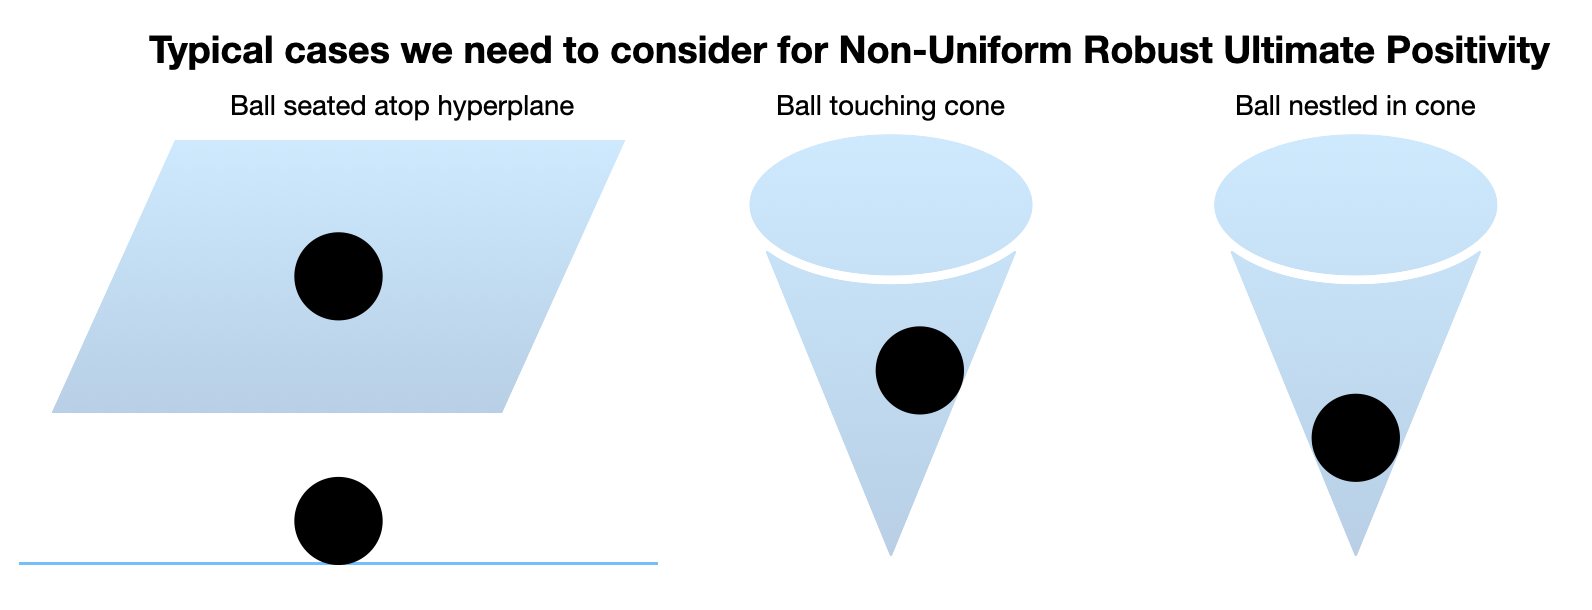
\includegraphics[width=\textwidth]{picture1.png}
\caption{Visual intuition}
\label{fig:geometricpicture}
\end{figure}
\subsection{Decidability at order three}
\label{section:decidability2}
In this section, we prove Theorem \ref{thm:decide2}. As before, the techniques naturally apply to lower orders, and we omit their explicit treatment. Recall equation \ref{eq:grouping} and the surrounding discussion:
\begin{equation}
u_n/n^d\rho^n = \begin{bmatrix}
{\color{red!70!black} \mathbf{q}_{dom}^T(n) } & \mathbf{q}_{res}^T(n)
\end{bmatrix}
\begin{bmatrix}
{\color{red!70!black} \mathbf{p}_{dom}} \\
\mathbf{p}_{res}
\end{bmatrix}
\end{equation}
The crucial first task is to check whether for all points $\mathbf{p'}$ in the neighbourhood, \\$\liminf_{n\in\naturals}\seq{\mathbf{q}_{dom}(n), \mathbf{p'}_{dom}} = \mu(\mathbf{p'}) \ge 0$. Although Ultimate Positivity is guaranteed for the points where the inequality is strict, the neighbourhood may intersect the critical region where $\mu = 0$. If there are no non-dominant terms, this is irrelevant; but otherwise decidability hinges on whether we can handle the intersection.

We make cases, based on the presence of a pair of complex conjugates among the dominant roots. If the dominant terms are all real, then $\seq{\mathbf{q}_{dom}(n), \mathbf{p'}_{dom}} \ge 0$ is the intersection of at most two halfspaces (of the form $z - |w| \ge 0$). The neighbourhood must lie entirely above the separating hyperplanes (ball atop hyperplane in Figure \ref{fig:geometricpicture}). The points where the neighbourhood is tangent to the planes have algebraic coordinates. The three polynomial equations for the three coordinates come from the facts that: (i) the point lies on the plane, (ii) the point lies on the surface of the neighbourhood, (iii) the gradient of $(\mathbf{p'} - \mathbf{p})^T\mathbf{M}(\mathbf{p'} - \mathbf{p})$ is along the normal to the plane. This gives us low-order, decidable instances of Ultimate Positivity.

Otherwise, there are no non-dominant terms, and $\seq{\mathbf{q}_{dom}(n), \mathbf{p'}_{dom}} = z + x\cos n\theta + y\sin n\theta$. We assume $\theta$ is not a rational multiple of $2\pi$ (can be detected, Theorem \ref{thm:abelian}): otherwise, the region where $\mu(\mathbf{p'}) \ge 0$ is again a finite union of halfspaces. Recall equation \ref{eq:liminfmin}. We get that $\mu(\mathbf{p'}) = z -\sqrt{x^2 + y^2}$. As shown in Figure \ref{fig:geometricpicture}, the critical region $\mu(\mathbf{p'})$ is a cone. Here, decidability follows by simply using Theorem \ref{thm:renegar} (Renegar) to evaluate the truth of this sentence in the First Order Theory of the Reals.
\begin{equation}
\label{eq:firsttask}
\chi := \forall \mathbf{p'}.~ (\mathbf{p'} - \mathbf{p})^T\mathbf{M}(\mathbf{p'} - \mathbf{p}) \le 1 \Rightarrow \mu(\mathbf{p'}) \ge 0
\end{equation}

\subsection{Hardness at order four}
\label{section:hardness2}
In this section, we prove Theorem \ref{thm:hardness2}. More precisely, given $t \in \mathcal{T}$, $0 < \rho < 1$, and a precision $\varepsilon > 0$, we will use the purported decidability of $\mathbf{S}$-Robust non-uniform Ultimate Positivity to approximate the maximal $\ell$ such that the set 
$$
E_{\ell\rho^n}(t) = \{s\in \reals: \ell\rho^n[nt - s] \le 1 \text{ for infinitely many } n\}
$$
is non-empty. We assume that $t$ is represented by an algebraic $p$, such that $\theta = 2\pi t = \arccos(p)$. The characteristic polynomial of our recurrence relation is $(X-1)(X-\nu)(X^2 - 2pX + 1)$, where $\nu = 1/\rho^2$. As in the previous reduction, we choose $\mathbf{S} = \frac{1}{2}(\mathbf{V}^{-1})^T\mathbf{V}^{-1}$ such that its translation $\mathbf{M}$ to the solution space is $1/2$ times the identity matrix. In the solution space, our neighbourhood is the ball of radius $\sqrt{2}$. We assume the solution to be $z + x\cos n\theta + y\sin n\theta + w\nu^n$.

We take the centre to be $(z = 2, x = 0, y= 0, w = -r), r > 0$. Observe that the neighbourhood intersects the cone $\mu = 0$ in the unit ring $z= 1, x^2 + y^2 = 1, w = -r$. This corresponds to the ball nestled in cone situation in Figure \ref{fig:geometricpicture}. The way to see this is by noting that the cone $z^2 = x^2 + y^2$ may be thought of as being carved by \textit{infinitely} many hyperplanes $z + x\cos \phi + y\sin \phi = 0$. The centre of the ball is at unit distance from each of them; going along the normal $(-1/\sqrt{2}, -\cos\phi/\sqrt{2}, -\sin\phi/\sqrt{2}, 0)$ for a distance of $\sqrt{2}$ gives the point of tangency $(1, -\cos\phi, -\sin\phi, -r)$. We need to crucially decide if Ultimate Positivity holds at \textit{each} of these points. 

This is not trivial: although Ultimate Positivity is known to be decidable for Simple LRS \cite{ouaknine2014ultimate}, as well as for low order LRS \cite{joeljames3}, the techniques therein assume that all input is algebraic, which is not the case here. Continuity arguments to interpolate from the decidable points likely don't work, as algebraic numbers form a measure $0$ countable subset of the uncountable reals.

Our problem is to decide whether, for each $\phi$, the inequality
\begin{equation}
\label{eq:ring}
1 -\cos(n\theta-\phi) \ge r\nu^n
\end{equation}
holds for all sufficiently large $n$. We reason exactly as we did in the previous section. Note $\nu = 1/\rho^2$, $[bx]_b = b[x]$, and the analogue of Lemma \ref{lemma:numerical}
\begin{lemma}
\label{lemma:numerical2}
For every $r, \varepsilon > 0$, we can compute $N$ such that,
$$1 - \cos x < r\nu^N  \Rightarrow 1- \cos x > (1 - \varepsilon)^2\frac{x^2}{2}$$
\end{lemma}

\textbf{Case YES}.
Since $\theta$ is not a rational multiple of $2\pi$, $n\theta - \phi$ can be a multiple of $2\pi$ at most once. We conclude that for every $\phi = 2\pi s$, $[n\theta-\phi]_{2\pi}^2 > 2r\nu^n$ for all sufficiently large $n$. In other words, for every $s$, $\left(\pi\sqrt{\frac{2}{r}}\right)\rho^n[nt - s] \le 1$ for only finitely many $n$. $\left(\pi\sqrt{\frac{2}{r}}\right)$ is thus an upper-bound for $\ell$.

\textbf{Case NO}.
There exists a $\phi_0$ such that $1 - \cos n\theta$ is infinitely often less than $r\nu^n$. Hence, for any $\varepsilon$, one can compute an $N$, and apply Lemma \ref{lemma:numerical2} on the infinitely many times $1 - \cos n\theta$ is small enough. We get that for every $\varepsilon$, there are infinitely many $n$, $(1-\varepsilon)^2[n\theta-\phi_0]_{2\pi}^2 < 2r\nu^n$. Since $\varepsilon$ is arbitrary, we can simplify as in the previous case, and argue that for $s_0$, $\left(\pi\sqrt{\frac{2}{r}}\right)\rho^n[nt - s_0] \le 1$ for infinitely many $n$. $\left(\pi\sqrt{\frac{2}{r}}\right)$ is thus a lower-bound for $\ell$.



\section{Uniform Robustness: Hardness at order five}
\label{section:hardness}
We shall prove Theorem \ref{thm:hardness} in this section. That is, given $\theta \in \mathcal{T}$ as defined in equation \ref{eq:keyset}, we shall give rational $\mathbf{a}, \mathbf{c}$ such that varying $\mathbf{S}$ while invoking $\mathbf{S}$-Robust Positivity decision procedures will enable us to approximate $L(t)$ and $L_\infty(t)$ to arbitrary precision.

\subsection{The hard sequence}
We assume $\theta$ is specified by $p \in \rationals$, $0 < |p| < 1$, such that $\theta = \frac{\arccos p}{2\pi}$. Our LRR $\mathbf{a}$ is such that the roots of the characteristic polynomial are $1, 1, 1, e^{2\pi i\theta}, e^{-2\pi i \theta}$, i.e. the characteristic polynomial is 
$
(X- 1)^3(X^2 - 2pX + 1)
$.

Here, 
$
u_n = \begin{bmatrix}
n^2 & n & 1 & \cos 2\pi n\theta & \sin 2\pi n\theta
\end{bmatrix}
\mathbf{p}
$, and we choose the input $\mathbf{S} = r^2(\mathbf{V}^{-1})^T\mathbf{V}^{-1}$ such that its translation $\mathbf{M}$ to the solution space is $r^2$ times the identity matrix.

We note that since both $p, q$ from the root $p + qi$ are rational, the linear map $\mathbf{V}^{-1}$ from the space of initialisations to the space of real exponential polynomial coefficients is also rational. In the solution space, we consider a ball of radius $r$ around $(r, 0, 1+\frac{r}{2}, -1, 0)$, i.e. by equation \ref{eq:crux}, we ask whether for all (but finitely many) $n$
\begin{align*}
rn^2 + \frac{r}{2} + 1 - \cos 2\pi n\theta \ge r\sqrt{n^4 + n^2 + 2} 
&\Leftrightarrow \frac{r}{2} + 1 - \cos 2\pi n\theta \ge r\left(\frac{n^2 + 2}{n^2 + \sqrt{n^4 + n^2 + 2}}\right) \\
&\Leftrightarrow 1 - \cos 2\pi n\theta \ge \frac{r}{2}\left(\frac{n^2 + 4 - \sqrt{n^4 + n^2 + 2}}{n^2 + \sqrt{n^4 + n^2 + 2}}\right)
\end{align*}
Simplifying to a slightly more indicative form, we ask whether for all (but finitely many) $n$
\begin{equation}
\label{eq:pivotal}
1 - \cos 2\pi n\theta \ge \frac{r}{2}\left(\frac{7n^2 + 14}{(n^2 + \sqrt{n^4 + n^2 + 2})(n^2 +4+  \sqrt{n^4 + n^2 + 2})}\right) = r\cdot Q(n)
\end{equation}

\subsection{Numerical analysis}
Inequality \ref{eq:pivotal} is pivotal to our reduction. We note that in the limit, the ratio of $Q(n)$ to $7/8n^2$ tends to $1$ from below. On the other hand, for small values of $[2\pi n\theta]_{2\pi}$, we shall approximate $1 -\cos 2\pi n \theta$ by $\frac{[2\pi n\theta]_{2\pi}^2}{2}$, which itself is tightly lower bounded by a constant multiple of $L(\theta)/n^2$. Thus, the universal validity of inequality \ref{eq:pivotal} hinges on how $r$ relates to $L$. We capture the crucial interdependence in the following technical lemma.

\begin{lemma}
\label{lemma:numerical}
Let $r < 100$. For every $\varepsilon > 0$, we can compute $N$ such that for all $n \ge N$,
\begin{enumerate}
\item $Q(n) > \frac{7(1-\varepsilon)^2}{8n^2}$
\item $1 - \cos x < \frac{7r}{8n^2} < \frac{700}{8N^2}  \Rightarrow 1- \cos x \ge (1 - \varepsilon)^2\frac{x^2}{2}$
\end{enumerate}
\end{lemma}

\subsection{Computing the Lagrange constant}
We use the purported decidability of $\mathbf{S}$-Robust Uniform Ultimate Positivity (does inequality \ref{eq:pivotal} hold for all but finitely many $n$?) to approximate $L_\infty(\theta)$ to arbitrary precision. 

\textbf{Case YES:} \\
Suppose indeed, for all but finitely many $n$,
$
1 - \cos 2\pi n\theta \ge r \cdot Q(n)
$ \\
$1 - \cos 2\pi n\theta$ is always upper bounded by $\frac{[2\pi n\theta]_{2\pi}^2}{2}$. In this case, we use Part 1 of Lemma \ref{lemma:numerical} to argue that for every $\varepsilon$, there exists an $N$ such that for all $n \ge N$,
$$
\frac{[2\pi n \theta]_{2\pi}^2}{2} > \frac{7r(1 - \varepsilon)^2}{8n^2} \Leftrightarrow n[n\theta] > (1 - \varepsilon)\frac{\sqrt{7r}}{4\pi}
$$
This allows us to conclude that $L_\infty(\theta) \ge \frac{\sqrt{7r}}{4\pi}$.

\textbf{Case NO:} \\
Suppose there exist infinitely many $n$ such that 
$
1 - \cos 2\pi n\theta < r \cdot Q(n)
$. \\
$r \cdot Q(n)$ is always upper bounded by $7r/8n^2$. In this case, we use the second part of Lemma \ref{lemma:numerical} on the infinitely many times $1 - \cos 2\pi n\theta$ is small enough. Here, for any $\varepsilon$, we will have infinitely many $n$ such that
$$
(1 - \varepsilon)^2 \frac{[2\pi n \theta]_{2\pi}^2}{2} < \frac{7r}{8n^2} \Leftrightarrow n[n\theta] < \left(\frac{1}{1-\varepsilon}\right)\frac{\sqrt{7r}}{4\pi}
$$ 
Thus, we can conclude that $L_\infty(\theta) \le \frac{\sqrt{7r}}{4\pi}$.

\subsection{Computing the Diophantine approximation type}
Here, we choose a precision $\varepsilon$, and compute the $N$ in Lemma \ref{lemma:numerical}. We use this $N$ to get an appropriate instance of $\mathbf{S}$-Robust Positivity for the hard LRS. 

Our goal is to be able to reason as follows, similar to the previous subsection, 
$$
\text{YES} \Rightarrow \inf_{n \ge N} n[n\theta] \ge (1 - \varepsilon)\frac{\sqrt{7r}}{4\pi}
$$
and
$$
\text{NO} \Rightarrow \inf_{n \ge N} n[n\theta] \le \left(\frac{1}{1-\varepsilon}\right)\frac{\sqrt{7r}}{4\pi}
$$
For the finite prefix $1$ to $N-1$, we can compute $n[n\theta]$ to arbitrary precision and compare with the purported lower/upper bounds for $L(\theta) = \inf_{n \in \naturals} n[n\theta]$.

Our query, therefore is
$$
\forall n \ge N.~ \mathbf{x_n}^T\mathbf{p} \ge r\sqrt{\seq{\mathbf{x_n}, \mathbf{x_n}}} 
$$
which, on taking $\mathbf{S} = r^2(\mathbf{V}^{-1})^T\mathbf{V}^{-1}$, is equivalent to
$$
\forall n \ge 0.~ \mathbf{A}^n(\mathbf{A}^N\mathbf{c}) \ge \max_{\mathbf{d} \in \ball_\mathbf{S}} \mathbf{A}^n(\mathbf{A}^N\mathbf{d})
$$
Let $\mathbf{c'} = \mathbf{A}^N\mathbf{c}$, $\mathbf{S'} = (\mathbf{A}^{-N})^T\mathbf{S}\mathbf{A}^{-N}$. Thus, our instance of robust Positivity is:
$$
\forall n \ge 0.~ \mathbf{A}^n\mathbf{c'} \ge \max_{\mathbf{d'} \in \ball_\mathbf{S'}} \mathbf{A}^n\mathbf{d'}
$$

Finally, we note that by replacing the coefficients $(r, 0, 1 + \frac{r}{2}, -1, 0)$ with  $(r, 0, 1 + \frac{r}{2}, \cos 2\pi\varphi, \sin 2\pi\varphi)$, the same reduction allows us to compute \textbf{inhomogeneous} Langrange constants and Diophantine approximation types.




\section{Extensions and Perspective}
As outlined at the outset, we contributed towards a sharp and comprehensive picture of what is \textit{decidable} about Robust Positivity Problems for real algebraic Linear Recurrence Sequences. We find it remarkable that number-theoretic analyses involving Diophantine approximation, which usually show up in the context of hardness, also play a significant role in our \textit{decidability} proofs! However, a rather conspicuous gap in our picture is the status of $\mathbf{S}$-Robust Non-uniform Ultimate Positivity at order $5$: this seems to require even more delicate analysis. 

An obvious, but possibly tedious future direction would be to tie up the book-keeping loose ends, and meticulously account for the complexity of our techniques. We chose to work with algebraic numbers; in settings involving rational numbers where scaling to integers and accessing an $\mathsf{PosSLP}$ oracle is viable, the complexity usually lies in $\mathsf{PSPACE}$. However, this might blow up significantly in the absence of efficient positivity testing for a different class of arithmetic circuit.

At a higher level, we note that we chose our norm to be based on the standard matrix inner product. It is interesting to investigate what kinds of decidability and hardness results hold for neighbourhoods specified using different norms. Perhaps, results could be universal across a wider class of norms, and there could be a profound underlying linear-algebraic reason whose discovery would be mathematically significant.

In the grand Formal Methods scheme, the study of Hyper-properties \cite{hyperproperties} is an exciting natural way robustness problems for Linear Dynamical Systems could fit in. Hyper-logics reason about sets of traces of an infinite time system, rather than a single trace. They gained importance as a means to verify security in view of attacks like Meltdown and Spectre. A quintessential hyper-property, for instance, would specify a reasonable notion of \textit{indistinguishability} of traces. In that regard, our notions of $\mathbf{S}$-Robust Positivity and $\mathbf{S}$-Robust Uniform Ultimate Positivity bear striking resemblance. Exploring deeper connections is a fascinating future research avenue.





\clearpage
\bibliography{main}
\clearpage

\appendix
\section{Appendix: Notation and Prerequisites}
\label{appendix:prelims}
For the purposes of discussing robustness, we shall use $\ball$ to denote the unit Euclidean ball in $\reals^\kappa$, centred at the origin. Similarly, we use $\ball_{\mathbf{S}}$ to denote the set of $\mathbf{d}$ such that $\mathbf{d}^T\mathbf{Sd} \le 1$. For real column vectors $\mathbf{x}, \mathbf{y}$, we use $\seq{\mathbf{x}, \mathbf{y}}$ to denote the inner product $\mathbf{x}^T\mathbf{y} = \mathbf{y}^T\mathbf{x}$. The notation $||\mathbf{x}||$ denotes the standard $\ell^2$-norm $\sqrt{\seq{\mathbf{x}, \mathbf{x}}}$.

Throughout this paper,  $\naturals$, $\integers$, $\rationals$, $\reals$, and $\complexes$ respectively denote the natural numbers, integers, rationals, reals, and complex numbers. $\alpha \in \complexes$ is said to be algebraic if it is a root of a polynomial with integer coefficients. Algebraic numbers form an algebraically closed field, denoted by $\algebraics$. We denote the field of real algebraic numbers by $\realalgebraics$.

This Appendix contains a brief initiation to this number field $\realalgebraics$ and $\algebraics$. The key takeaways are that the usual arithmetic as well as polynomial root computation can be carried out with perfect precision, and that the First Order Theory of the Reals $\seq{\reals; +, \cdot, \ge, 0, 1}$ is a decidable logical system powerful enough to fit our purposes.

\subsection{Algebraic Numbers: Arithmetic}
For an algebraic number $\alpha$, its defining polynomial $p_\alpha$ is the unique polynomial in $\integers[X]$ of least degree such that the GCD of its coefficients is $1$ and $\alpha$ is one of its roots.
Given a polynomial $p \in \integers[X]$, we denote the length of its representation by $\text{size}(p)$; its height, denoted by $H(p)$, is the maximum absolute value of the coefficients of $p$; $d(p)$ denotes the degree of $p$. The height $H(\alpha)$ and degree $d(\alpha)$ of $\alpha$ are defined to be the height and degree of $p_\alpha$.

For any $p \in \integers[X]$, the distance between distinct roots is effectively lower bounded in terms of its degree and height \cite{mignottecon}.
This bound allows one to represent an algebraic number $\alpha$ as a 4-tuple $(p,a,b,r)$ where $p$ is the defining polynomial, and $a+bi$ is a rational approximation of sufficient precision $r\in\rationals$. We use $\text{size}{\alpha}$ to denote the size of this representation, i.e., number of bits needed to write down this 4-tuple.

Given a polynomial $p\in \integers[X]$, one can compute its roots in polynomial time \cite{findroots1operate1}. Recently, implementations of algorithms to factor polynomials in $\algebraics[X]$ have been verified \cite{factor-algebraic}. Given $\alpha$, $\beta$ two algebraic numbers, one can always compute the representations of $\alpha+\beta$, $\alpha\beta$, $\frac 1 \alpha$, $\Re(\alpha)$, $\Im(\alpha), |\alpha|$, and decide $\alpha = \beta$, $\alpha > \beta$ in polynomial time wrt the size of their representations. \cite{findroots1operate1,findroots2operate2}.

\subsection{First Order Theory of the Reals}
This logical theory reasons about the universe of real numbers, and is denoted $\seq{\reals; +, \cdot, \ge, 0, 1}$. That is, variables take real values; terms can be added and multiplied, we have the comparison predicate, and direct access to the constants $0$ and $1$. Thus, our propositional atoms are inequalities involving polynomials with integer coefficients. With existential quantifiers and polynomials, we can thus express algebraic constants too. Formally, we have access to only the existential quantifier, negation, and disjunction; however, this can express the universal quantifier and all other Boolean connectives as well.

Variables are either quantified or free. Remarkably, the First Order Theory of the Reals admits quantifier elimination: for any formula $\chi(\mathbf{x})$, whose free variables are $\mathbf{x}$, there exists an \textbf{equivalent} formula $\psi(\mathbf{x})$ that does not contain any quantified variables. The following result is relevant to us.
\begin{theorem}[Renegar \cite{renegar}]
\label{thm:renegar}
Let $M \in \naturals$ be fixed. Let $\chi(\mathbf{x})$ be a formula with fewer than $M$ variables in total. There exists a procedure that returns an equivalent quantifier-free formula $\psi(\mathbf{x})$ in disjunctive normal form. This procedure runs in time polynomial in the size of the representation of $\chi$.
\end{theorem} 
\section{Appendix: Ostrowski Numeration System}
\label{appendix:ostrowski}

In this appendix, we prove Lemma \ref{lemma:existsreal}. We state number-theoretic properties of the continued fraction representation and Ostrowski Numeration System without proof. We refer the reader to \cite{bourla2016ostrowski} for a more detailed exposition, and we closely follow the discussion surrounding \cite[Propositions 1.1, 2.1]{berthe2022dynamics} in our own proof. We first prove a slightly simpler statement.

\begin{lemma}
\label{lemma:existsreal2}
For every irrational number $x$, strictly decreasing real positive function $\psi$, and interval $\mathcal{I} = [\alpha, \beta] \subset [0, 1], ~ \alpha \ne \beta$, there exists $y \in \mathcal{I}$ such that $[nx - y] < \psi(n)$ for infinitely many $n$.
\end{lemma}
\begin{proof}
Without loss of generality, we can assume that $x \in (0, 1)$. Consider the continued fraction representation of $x$: $[0; a_1, a_2, a_3, \dots]$
$$
x = \cfrac{1}{a_1 + \cfrac{1}{a_2 + \cfrac{1}{a_3 + \cfrac{1}{\ddots}}}}
$$
where $a_1, a_2, a_3, \dots \in \naturals$. Let the rational approximation of $x$ obtained by truncating the expansion at the $k^{th}$ level be $\frac{p_k}{q_k}$, i.e. $\frac{p_1}{q_1} = \frac{1}{a_1}$, and so on. Let $\theta_k = q_k x -p_k$. We have that $|\theta_k| = (-1)^k\theta_k$. It is well known that $|\theta_k| < 1/q_k$. We define $q_{-1} = p_0 := 0$, and $p_{-1} = q_0 := 1$, so that for $k \ge 1$, the following recurrences hold:
$$
p_k = a_kp_{k-1} + p_{k-2}, ~ q_k = a_kq_{k-1} + q_{k-2}
$$
We thus have that $q_k \ge \left(\frac{1 + \sqrt{5}}{2}\right)^k = \phi^k$.

\begin{proposition}
\label{prop:absconv}
Let irrational $x$ and its continued fraction representation $[0; a_1, a_2, a_3, \dots]$ be as above. The infinite series 
$$
\sum_{i=1}^\infty a_i |\theta_{i-1}|
$$
converges.
\end{proposition}

\begin{proposition}[Ostrowski Numeration System]
\label{prop:numsys}
Every real number $y \in [0, 1)$ can be written uniquely in the form
$$
y = \sum_{i=1}^\infty b_i |\theta_{i-1}| = \sum_{i=1}^\infty (-1)^{i-1}b_i \theta_{i-1} 
$$
where $b_i \in \naturals$ $b_i \le a_i$ for all $i \ge 1$. If for some $i$, $a_i = b_i$, then $b_{i+1} = 0$. $a_i \ne b_i$ for infinitely many odd, and infinitely many even indices $i$.
\end{proposition}

We prove Lemma \ref{lemma:existsreal2} by using the free choice of $b_i$ in this system to construct appropriate $y$. We first handle the issue of placing $y$ in the correct interval $[\alpha, \beta]$. Let $\beta - \alpha = \delta$. We use Proposition \ref{prop:absconv} to argue that there exists a suffix of the infinite series, such that changing the suffix does not change the real number it represents by more than $\delta/2$. Then, we can simply fix the corresponding prefix of $(\alpha + \beta)/2$ to be the prefix of $y$.

Once this prefix is locked in, our strategy is to set $b_i$ to $0$ in even positions, and $1$ in some odd positions, to ensure that for sufficiently large $k$, $n_k = \sum_{i=1}^k b_i (-1)^{i-1}q_{i-1}$ is positive, and increasing in $k$.

Now, notice that since $b_i, p_i$ are all integers, for any $y$,
\begin{align*}
[n_kx - y] &= \left[\sum_{i=1}^k b_i (-1)^{i-1}q_{i-1}x - \sum_{i=1}^k b_i (-1)^{i-1}p_{i-1} - y\right] \\
&= \left[\sum_{i=1}^k b_i (-1)^{i-1}\theta_{i-1} - y\right] \\
&= \left[- \sum_{i=k+1}^\infty b_i (-1)^{i-1}\theta_{i-1} \right] = \sum_{i=k+1}^\infty b_i |\theta_{i-1} |\\
&< \sum_{i=k+1}^\infty b_i \frac{1}{q_{i-1}} \le \sum_{i=k+1}^\infty b_i \frac{1}{\phi^{i-1}} \le \frac{c}{\phi^k}
\end{align*}

Note that the last constant $c$ can be set independently of the choice of which $b_i$ are $1$, and which are $0$: it comes from the convergence of the geometric sum. We now make the choice of where to set $b_i=1$. To conclude the proof, we shall show that given a decreasing function $\psi$, we can ensure that for infinitely many distinct $n_k$, 
$$[n_k x - y] < \frac{c}{\phi^k} \le \psi(n_k) = \psi\left(\sum_{i=1}^k b_i (-1)^{i-1}q_{i-1}\right)$$.

The first inequality is guaranteed. Suppose the second inequality does not hold. Then, from $i = k$ onwards, we keep assigning $b_i := 0$. This holds $n_k$ constant as $k$ increases, but decreases $\frac{c}{\phi^k}$. Eventually, the second inequality will indeed hold. After this point, for the next odd $i$, we can set $b_i$ to $1$, and get a new $n_k$. We continue this ad infinitum, and we are done.
\end{proof}

Now, to get infinitely many \textit{even} $n$, apply Lemma \ref{lemma:existsreal2} with $2x$, $[a, b]$, $\psi_0(n) = \psi(2n)$. For some choice of $y$, there will be infinitely many $n$ such that $[2nx - y] < \psi_0(n) = \psi(2n)$. To get infinitely many \textit{odd} $n$, we can take a subset of the interval, and shift it by $x$. Take $\psi_1(n) = \psi(2n+1)$. For some choice of $y - x$, there will be infinitely many $n$ such that $[n(2x) - (y-x)] = [(2n+1)x - y] < \psi_1(n) = \psi(2n+1)$.


\end{document}